
\section{Auto-Tools}
\label{sect:esan}
\subsection{Introduction to the Autotools}
Introduction to the Autotools is a series of tutorial videos made by David A. Wheeler\cite{wheeler2012autopart1,wheeler2012autopart2,wheeler2012autopart3}.
Autotools is a collection of various tools designed to make the use of compiling source, and Make in particular, easier~\citep{wheeler2012autopart1}. Autotools can help creating platform independent sources~\citep{wheeler2012autopart1}. AutoMake, part of Autotools,  assists in solving dependencies of source files. It also supports the use of nested structures without the user having to create complicated makefiles~\cite{wheeler2012autopart2}. Autotools can be used to help cross-compilation on platforms~\citep{wheeler2012autopart2}. Autotools are bundled with methods to resolve and locate dependencies on a system.
Autotools supports the recursive make paradigm (although this should not be used, see \ref{sec:recursivemake})~\citep{wheeler2012autopart3}. It's advisable to prefer a large Makefile.am as opposed to a recursive build structure~\citep{miller1998recursive,wheeler2012autopart3}.

\subsection{Recursive Make Considered Harmful}
\label{sec:recursivemake}
Peter Miller wrote an article about the problems he noticed in the usage of the Make\cite{miller1998recursive}. Most notably the problems that originate from the Recursive Make paradigm.
Image~\ref{fig:peter_miller}\footnote{Source: \url{http://miller.emu.id.au/pmiller/}} shows him over the years.
\begin{figure} \centering
\captionsetup[subfigure]{labelformat=empty}
\begin{subfigure}{0.19\textwidth}

\includegraphics[width=\textwidth]{images/peter_miller_2009.jpg}
\caption{2009}
\end{subfigure}
\begin{subfigure}{0.19\textwidth}
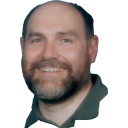
\includegraphics[width=\textwidth]{images/peter_miller_2003.png}
\caption{2003}
\end{subfigure}
\begin{subfigure}{0.19\textwidth}

\includegraphics[width=\textwidth]{images/peter_miller_1993.png}
\caption{1993}
\end{subfigure}
\begin{subfigure}{0.19\textwidth}

\includegraphics[width=\textwidth]{images/peter_miller_1981.png}
\caption{1981}
\end{subfigure}
\begin{subfigure}{0.19\textwidth}
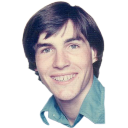
\includegraphics[width=\textwidth]{images/peter_miller_1975.png}
\caption{1975}
\end{subfigure}
\caption{Peter Miller over time}
\label{fig:peter_miller}
\end{figure}

The author describes several problems with recursive make and attributes these to make not being allowed to do it's work. Make resolves dependencies to determine what requires rebuilding and what doesn't. By the principles of recursive make this becomes impossible. Instead the author propagates the use of full project makefiles of a modular format. A user must then rebuild the entire project. This allows make to properly analyze the DAG for dependencies and determining which parts need to be updates.

The indexing cost of this is negligible when compared to the cost of over-building or rebuilding in order to prevent bugs and race conditions. This cost becomes even more negligible when the user takes into account the time saved with debugging. The recursive make paradigm is prone to several bugs and race-conditions. By removing recursive make from the equation time can be saved during development. E.g. time spend debugging the system as opposed to debugging the code.

The full project make also allows make to make full use of the option of parallel building. Because the entire DAG is available make can work on both ends simultaneously, with recursive make this is impossible because make is not aware of the greater scope of the dependencies.

\subsubsection{Present Day}
A lot of the reasons and arguments in favor of recursive makes are no longer applicable on current computers. Memory has become cheap and processing power too. With current design philosophies going towards greater parallelism it seems that the argument to allow make a full DAG are still applicable. The assumed un-manageability of big makefiles is stopped by the appearance of build tools which automate the process.


